\documentclass[12pt]{article}

\usepackage{times,fullpage,xspace,fancyhdr,url}
\usepackage[pdftex]{graphicx}
\usepackage[pdftex,
            a4paper,
            colorlinks=true,
            urlcolor=black,
            linkcolor=black,
            citecolor=black,
            bookmarksopen=false,
            bookmarksnumbered=true,
            pdfstartview=FitH]{hyperref}

\usepackage{graphicx}
\usepackage{xspace,color}
\pdfcompresslevel=9
\newcommand{\leaguename}{RoboCup Standard Platform League (NAO) }
\hypersetup{
  pdftitle={\leaguename Technical Challenges},
  pdfauthor={Technical Committee},
}
\usepackage[latin1]{inputenc}
\usepackage{amsmath}

% comment 'disable' in to disable all the todo notes :)
\usepackage
[
%disable
]{todonotes}

\sloppy
\newcommand{\ie}{\mbox{i.\,e.}\xspace}
\newcommand{\eg}{\mbox{e.\,g.}\xspace}
\newcommand{\cf}{\mbox{cf.}\xspace}
\newcommand{\comment}[1]{\marginpar{\pdfannot width 4in height .5in depth 8pt {/Subtype /Text /Contents (#1)}}}
\newcommand{\inparagraph}[1]{\paragraph{#1\hspace{-1em} }}


% some colors
\definecolor{orange}{rgb}{1,0.5,0}
\definecolor{red}{rgb}{1,0,0}
\definecolor{green}{rgb}{0,1,0}

\title{\leaguename\\Technical Challenges}
\author{RoboCup Technical Committee}
\date{(2019 technical challenge rules, as of \today)}

\setlength{\parindent}{0pt}
\setlength{\parskip}{12pt plus 6pt minus 3 pt}
\setcounter{tocdepth}{1}
\widowpenalty=10000
\clubpenalty=10000

\pagestyle{fancy}
\lhead{}
\chead{}
\rhead{}
\lfoot{}
\cfoot{}
\rfoot{}

\renewcommand{\headrulewidth}{0.4pt}
\renewcommand{\footrulewidth}{0.4pt}

\newcommand{\TotalWidth}{7.4~m\xspace}
\newcommand{\TotalLength}{10.4~m\xspace }
\newcommand{\KickOffAutoTime}{45 seconds\xspace}
\newcommand{\FreeKickTime}{30 seconds\xspace}
\newcommand{\FreeKickRadius}{0.75m\xspace}
\newcommand{\PenaltyKickTime}{30 seconds\xspace}

% needed to align an image and text correctly side by side
\newcommand{\imagebox}[1]{\raisebox{2ex}{\raisebox{-\height}{#1}}}

\begin{document}

\maketitle

At RoboCup 2019, the Standard Platform League will hold two different technical challenges, which are described in this document.

The scores earned in each challenge will vary in magnitude. Hence, they must be scaled before calculating the overall technical challenge rankings. Teams who do not participate in a challenge will receive 0 points for that challenge. The team with the highest total score for a challenge will get 25 points for that challenge, while the team with the lowest total score for a challenge will get 5 points for that challenge. A linear equation will then be fit to these two points, and each other participating team in that challenge will gain points for that challenge based on this equation.

For both challenges, no changes of code or configuration are allowed for any participating team after the first team starts the challenge.

Questions or comments on the technical challenge rules should be mailed to \url{rc-spl-tc@lists.robocup.org}.

\vfill
\tableofcontents
\setcounter{tocdepth}{3}
\thispagestyle{fancy}
\clearpage
\cfoot{\thepage}
\setcounter{page}{1}

\section{Open Research Challenge}

The open research challenge serves as a supplement for the posters that are mentioned in Appendix A.1 of the official rules document. It should be especially used to demonstrate a team's own contributions to the state of the art in the league. In its procedure, it is similar to the Open Challenges that have been held until RoboCup 2014.

Each team that wishes to compete in this challenge \emph{must} send a short, maximum one page document describing what kind of demonstration they do during their presentation time to the technical committee by \textbf{June 17, 2019}. This document will be used to judge whether the presentation is adherent to the rules listed below. The technical committee will review the documents and notify teams whether their proposed demonstrations are acceptable. Teams who do not submit this description by the deadline will not be allowed to compete in this challenge.

Each team will be given three minutes of time on an SPL field for a presentation.

\begin{itemize}
\item The presentation must be strongly related to the scope of the league. Irrelevant demonstrations, such as dancing and debugging tool presentations, are not allowed.
\item The presentation should involve a demonstration using (any number of) real NAO robots (\ie presentations without practical demonstration are assumed to be ranked lower than others). The use of simulation is also possible, but only if the demonstrated research is not related to topics inherently interacting with the real world (\eg walking, perception) and it is guaranteed, \eg through interactivity, that it is actually a simulation and not a video, and the simulated robot resembles a NAO robot (\ie it does not have obvious capabilities that the NAO does not have).
\item Teams have three minutes for their presentation. At most one additional minute may be used for initial setup. Any demonstration deemed likely to require excessive time will be disallowed by the technical committee.
\item Teams may use extra objects on the field as part of their demonstration. \emph{Robots other than the NAOs may not be used.}
\item A demonstration must \emph{not} mark or damage the field. Any demonstration deemed likely to mark or damage the field will be disallowed by the technical committee.
\item A demonstration may \emph{not} modify the NAO robots.
\end{itemize}

\subsection{Score}

The winner will be decided by a vote among the SPL teams using the Borda count mechanism (\url{http://en.wikipedia.org/wiki/Borda_count}). Each SPL team will vote for their top 10 teams in order (excluding themselves). Teams are encouraged to evaluate the performance based on the following criteria: technical strength, novelty, expected impact and relevance to RoboCup, quality of the presentation. At a time decided by the designated referee, within one hour of the last demonstration if not otherwise specified, the captain of each team will submit his or her team's rankings by filling out an online form at \url{https://forms.gle/eiRJRqaJJZWTituV7}. Any points awarded by a team to itself will be disregarded. The points awarded by the teams will be summed and thus form the score of this challenge which is then converted according to the formula described in the preface of this document.

\newpage

\section{Directional Whistle Challenge}

The intention of this challenge is to investigate the possibilities of localizing the point where the referee whistle is blown.

\subsection{Setup}
\label{sec:dwc:setup}
Each participating team provides a number of robots from \(1\) to \(5\) for this challenge. The choice of the actual number of robots is up to the team, but it may affect the final ranking (\cf Section~\ref{sec:dwc:score}). Each robot has to wear a jersey with a number from the set \(\{1,2,3,4,5\}\). They are placed on predefined spots on a regular SPL field and oriented in some predefined orientation (per spot), where each spot corresponds to a jersey number (\cf Figure~\ref{fig:dwc:poses}). Thus, if a team chooses to use less than 5 robots, they can select which subset of poses is used by the jersey numbers of the robots they provide.

\begin{figure}[b!]
  \centerline{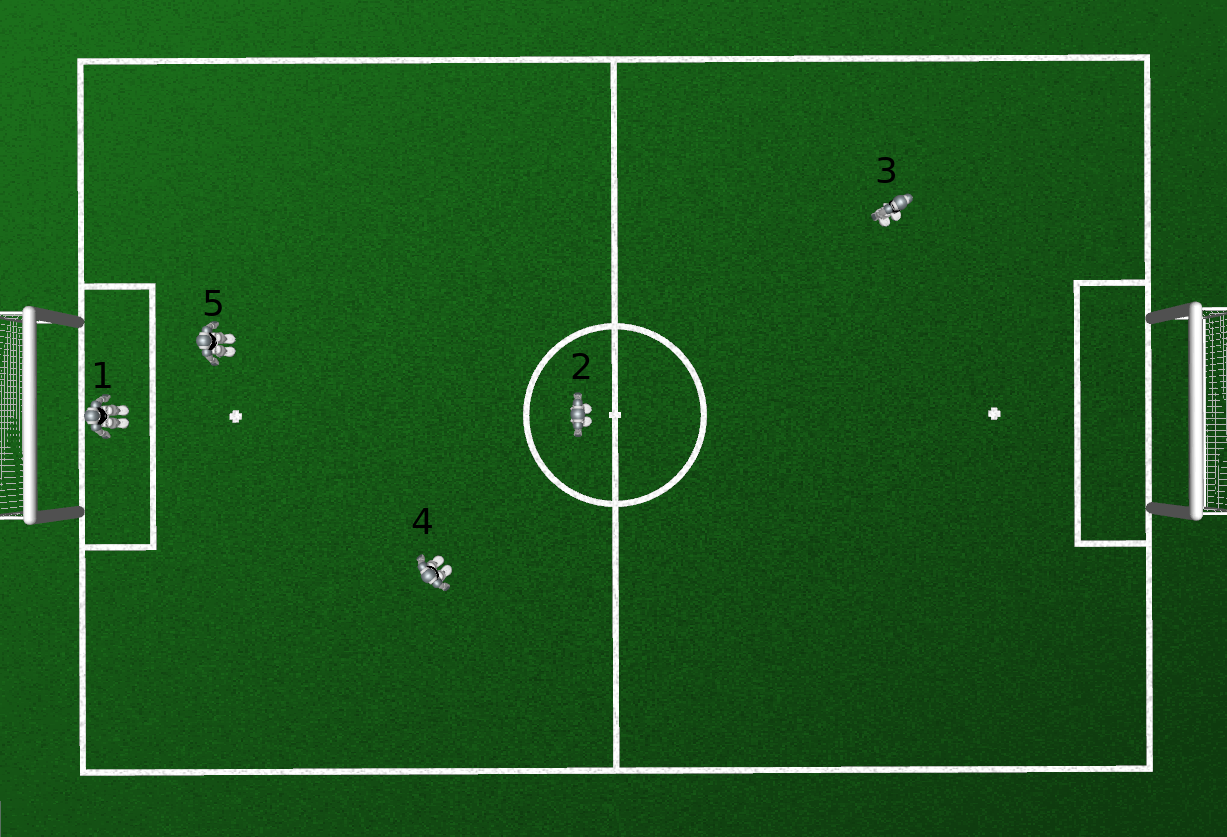
\includegraphics[width=\columnwidth]{figures/dwc-poses}}
  \caption{The poses that robots will be placed at during the challenge, based on their jersey number. Robot 3 is oriented towards the penalty cross, robot 4 towards the center of the field. The exact coordinates are specified in the \texttt{Config/robotPoses.json} file of the testing application.}
  \label{fig:dwc:poses}
\end{figure}

To evaluate the success of the challenge, at least one of the robots must be connected to a wireless network (with the same settings as in normal games) such that it can send messages to a testing application\footnote{available at \url{https://github.com/bhuman/DirectionalWhistleTester}} running on a separate computer. Wireless communication between the robots using the provided network is also allowed and is not subject to the usual restrictions, \eg robots may send more than one message per second in this challenge.

The robots have to be in a manually penalized state when handed over to the TC. The GameController will not be used in this challenge. The robots will be manually unpenalized with a single chest button press (not necessarily at the same time for all robots) after they have been placed on the field by TC members.

\subsection{Procedure}
\label{sec:dwc:procedure}
The challenge is conducted for each team separately after each other. After the robots have been set up, a ``referee'' blows a whistle from \(8\) different points (that are the same for all teams). Some of them are on the same field as the robots and others are on neighboring fields.

In the moment the referee blows the whistle, the operator of the testing application presses a button so that incoming messages will be associated with the current whistle position and the starting time of the attempt can be tracked. Following the whistle, the testing application will accept the first message it receives until up to \(5\) seconds after the attempt has started. Messages that are received in between attempts will be ignored by the testing application. After \(5\) seconds, the attempt is over and the referee will proceed to the next whistle position.

As message format, the SPL standard message (as distributed with the GameController) is used, where some fields have a different meaning for the purpose of this challenge:
\begin{itemize}
\item The \texttt{version} field must be set to 255 such that messages between robots and messages from robots to the testing application can be distinguished.
\item The \texttt{fallen} field should contain a value of 0 if the robots assume the whistle has been from another field and a nonzero value if they think the whistle has been blown on their field.
\item The first two entries of the \texttt{pose} field should contain the 2D position of the whistle on the ground in Cartesian coordinates in millimeters, in the same coordinate system that the \texttt{pose} field normally uses (which is the same coordinate system in which the robot poses will be specified).
\end{itemize}
The message will be used by the testing application to automatically calculate the score, as it has access to the list of positions occupied by robots and the list of points from which the whistle is blown. All other parameters of the network communication (IP address, UDP port, broadcast etc.) are the same as for SPL standard messages between robots, such that no separate networking code is necessary. Note that since UDP communication is used, it might be beneficial to report a detection multiple times (although not too often).

Note that although the message contains Cartesian coordinates, the scoring uses polar coordinates to better model the deviation of measurements. For this, the pose of the robot on the field that is closest to the actual whistle is used as reference pose. The testing application will automatically do the necessary transformations.

The robots are only allowed to move their heads during the challenge. All other motions (especially locomotion) are not allowed and result in the disqualification of that team from this challenge. Just as in the normal rules, any sports whistle is allowable. It can be assumed that the whistle will be blown by a standing person.

\subsection{Score}
\label{sec:dwc:score}
Each whistle attempt contributes to the score of a team based on three aspects:
\begin{description}
\item[Whether the decision between ``same field'' and ``other field'' is correct:] \(1\) point is awarded if it is correct, \(0\) otherwise.
\item[Angular precision:] \(1\) point is awarded if the absolute value of the calculated angle is within \(5^\circ\) of the actual direction. Between \(5^\circ\) and \(30^\circ\) deviation, the number of points scales linearly between \(1\) and \(0\) (\eg a deviation of \(15^\circ\) yields \(0.6\) points). Deviations larger than \(30^\circ\) yield no points.
\item[Distance precision:] \(1\) point is awarded if the calculated distance is within a \(\pm5\%\) range of the actual distance. Between \(5\%\) and \(30\%\) deviation, the number of points scales linearly between \(1\) and \(0\) (\eg a deviation of \(20\%\) of the actual distance yields \(0.4\) points). Deviations larger than \(30\%\) of the actual distance yield no points.
\end{description}
That is, if the whistle is correctly detected as being on the same field, the direction has a deviation of \(10^\circ\) and the distance has a deviation of \(17.5\%\), \(1+0.8+0.5=2.3\) points are awarded. If after \(5\) seconds there has been no reaction from the robot, the attempt is over, no points are awarded, and the whistle is blown from the next of the \(8\) points.

The scores of all \(8\) attempts are added together to form a number between \(0\) and \(24\) which is the total score of the team. In case of a tie (after transforming the score of this challenge to the overall challenge score and combining it with the Open Research Challenge), teams which used less robots in this challenge will be ranked superior.

\end{document}
